\begin{figure}[htbp]
	\centering
	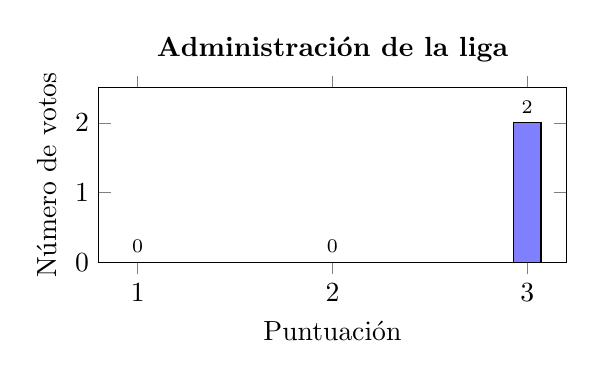
\begin{tikzpicture}
		\begin{axis}[title={\textbf{Administración de la liga}}, width=0.62\textwidth, ybar, bar width=10pt, height=3.8cm, ymin=0, ymax=2.5, xlabel={Puntuación}, ylabel={Número de votos}, xtick={1,2,3}, symbolic x coords={1,2,3}, nodes near coords, every node near coord/.append style={font=\scriptsize}]
		\addplot[fill=blue!50] coordinates {(1,0) (2,0) (3,2)};
		\end{axis}
	\end{tikzpicture}
	\caption{Valoración de la administración de la liga}
	\label{fig:admin_col}
\end{figure}

En la Figura \ref{fig:admin_col} vemos cómo la administración y gestión deportiva a través de la aplicación no es ni lo mejor ni lo peor. No habría que aplicar mejoras respecto a lo existente, pero podemos añadir nuevas funcionalidades que faciliten el trabajo de los administradores.

\begin{figure}[htbp]
	\centering
	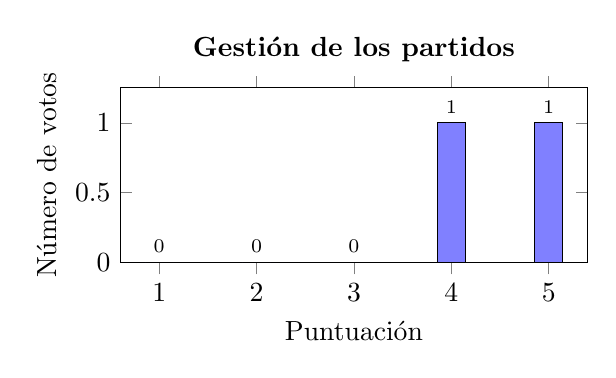
\begin{tikzpicture}
		\begin{axis}[title={\textbf{Gestión de los partidos}}, width=0.62\textwidth, ybar, bar width=10pt, height=3.8cm, ymin=0, ymax=1.25, xlabel={Puntuación}, ylabel={Número de votos}, xtick={1,2,3,4,5}, symbolic x coords={1,2,3,4,5}, nodes near coords, every node near coord/.append style={font=\scriptsize}]
		\addplot[fill=blue!50] coordinates {(1,0) (2,0) (3,0) (4,1) (5,1)};
		\end{axis}
	\end{tikzpicture}
	\caption{Valoración de la gestión de los partidos}
	\label{fig:referee_col_0}
\end{figure}

Según la Figura \ref{fig:referee_col_0}, la gestión de los partidos parece ser excelente. Aunque cabe recalcar que los árbitros utilizan diversas aplicaciones para gestionar los partidos: tanto para arbitrar un partido como para anotar los resultados. Por ello existe la necesidad de hacer un sistema unificado para todos los interesados.

\begin{figure}[htbp]
	\centering
	\begin{tikzpicture}[scale=0.75]
		\pie[text=legend, hide number, sum=auto, every pie/.style={font=\scriptsize}]{2/Tablet (2 votos)}
	\end{tikzpicture}
	\caption{Dispositivo utilizado para rellenar el acta}
	\label{fig:referee_col_1}
\end{figure}

La Figura \ref{fig:referee_col_1} nos confirma la necesidad del sistema multiplataforma al observar el uso de tablets por parte de los árbitros para rellenar el acta de los partidos.

\begin{figure}[htbp]
	\centering
	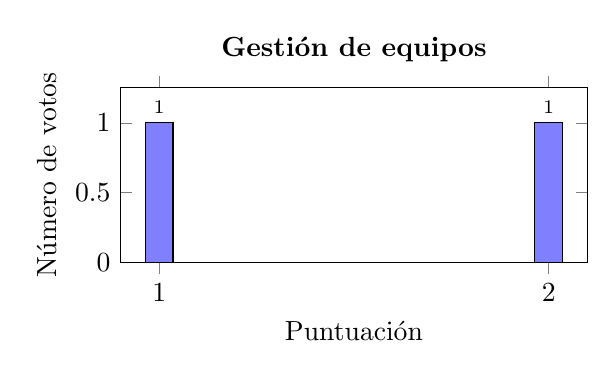
\begin{tikzpicture}
		\begin{axis}[title={\textbf{Gestión de equipos}}, width=0.62\textwidth, ybar, bar width=10pt, height=3.8cm, ymin=0, ymax=1.25, xlabel={Puntuación}, ylabel={Número de votos}, xtick={1,2}, symbolic x coords={1,2}, nodes near coords, every node near coord/.append style={font=\scriptsize}]
		\addplot[fill=blue!50] coordinates {(1,1) (2,1)};
		\end{axis}
	\end{tikzpicture}
	\caption{Valoración de la gestión de equipos}
	\label{fig:captain_col}
\end{figure}

En la Figura \ref{fig:captain_col} vemos como la opinión respecto a la gestión de equipos es muy baja. Esto nos lleva a deducir que puede ser interesante añadir funcionalidades para mejorar la interactividad y participación de los usuarios a la hora de gestionar los equipos deportivos.